\documentclass[a4paper]{article}

\usepackage[utf8]{inputenc}
\usepackage[T1]{fontenc}
\usepackage{textcomp}
\usepackage[english]{babel}
\usepackage{amsmath, amssymb}
\usepackage{caption}
\usepackage{minted}


% figure support
\usepackage{import}
\usepackage{xifthen}
\pdfminorversion=7
\usepackage{pdfpages}
\usepackage{transparent}
\newcommand{\incfig}[1]{%
	\def\svgwidth{\columnwidth}
	\import{./figures/}{#1.pdf_tex}
}

\newenvironment{code}{\captionsetup{type=listing}}{}

\pdfsuppresswarningpagegroup=1

\title{CS 213 - Data Structures and Algorithms}
\begin{document}
\maketitle	
\section{Introduction}
Twitter's banner problem - the agenda is to analyze this problem and
work towards a solution. 

CEO of twitter - Parag Agarwal - his student. Well anyway. What's the
problem at hand? People post content on twitter. There's some four people
on the banner page of twitter. Those four people will show up to scrapers etc.

Problem: Place "most popular  posts on the top page dynamically - updated every five-ish minutes or so."

If some folk says something super-interesting that has the potential
to go super-viral, then you want to push that person's post onto the
banner page.

So, consider an array of popularity indices. You as a programmer need
to process this. We will work with toy models only - no full sized
user bases and all.

We want to get the most popular from the list. $\mathcal{O}(n)$ to
get \texttt{max},  then there's going to be a hole to plug. One approach - 
sort the list, pop from the stack. This way no holes to be dealt with.
Problem with sorting (in this particular situation) - if a super-interesting post comes in - we will
not be in a position to dynamically adjust the stack to prioritize it.
Also, sorting is something like $\mathcal{O}(n^2)$ - number of cycles
doubles in order of magnitude.  

\begin{figure}[h]
	\centering
	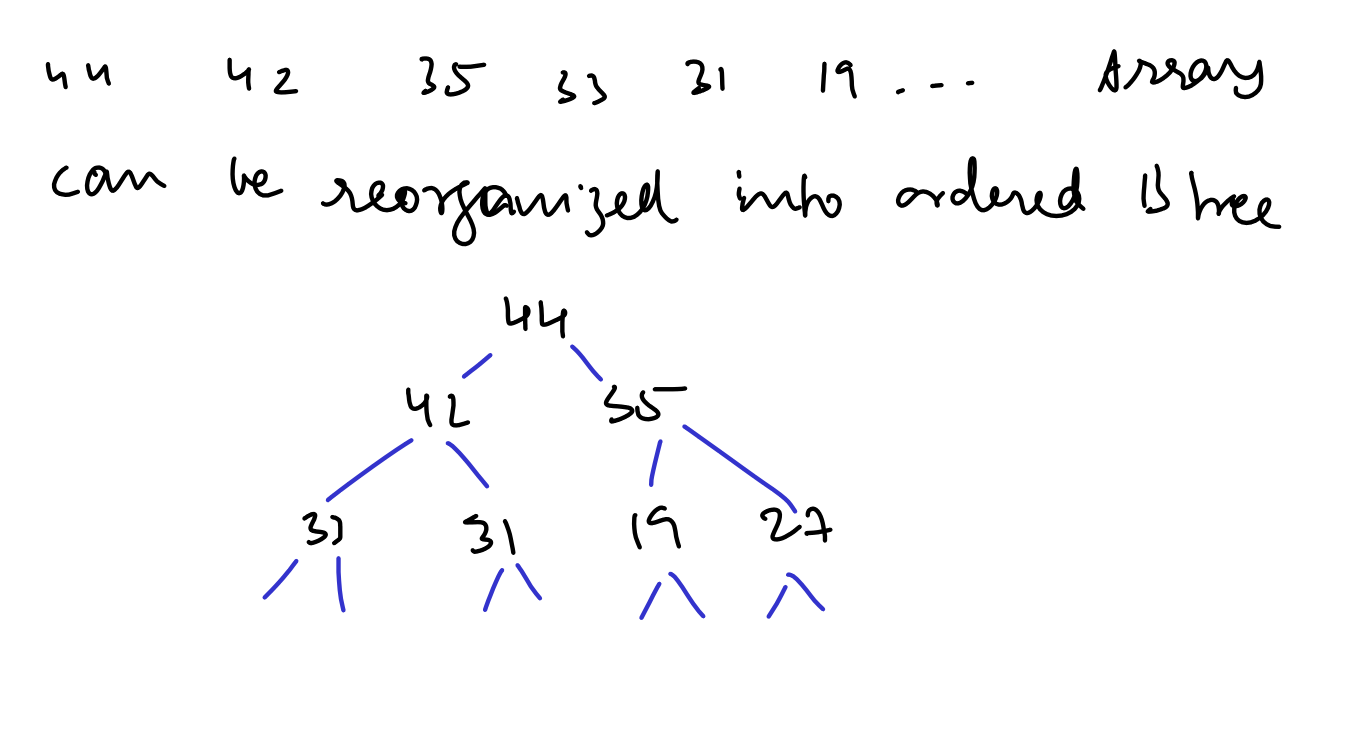
\includegraphics[width=0.8\textwidth]{figures/btree.png}
	\caption{figures/btree.png}
	\label{fig:Ordered binary tree - root, left child, right child}
\end{figure}
The data can be reorganized into another data structure that is more
convenient w.r.t insertions, searching etc. See the above figure.
That is a complete, ordered binary tree (ordered $\implies$ left child
and right child are  distinct for each node, binary $\implies$ two leaves per node, $2^{i}$ nodes in level $i$).

Internally, a binary tree such as this is still stored as an array.
If we want the right child of $j$, we only need realize $j \to 2j+1$.,
which is like ultra easy for the computer.

\begin{itemize}
	\item Right child: $j\to 2j+1$ 
	\item Parent: $k\to \frac{k}{2}$
\end{itemize}
The tree has a 
\begin{itemize}
	\item Structure property: it's a complete B tree
	\item Comparison property: the internal array is sorted - reflects in the B Tree representation
\end{itemize}

So, how would we go about handling the banner problem? The problem
is finding the most popular, next most popular and so on\ldots And
the twist is that there are insertions and deletions happening
dynamically in the internal array. 

So, the first part is \textit{Extract max}.
\begin{figure}[h]
	\centering
	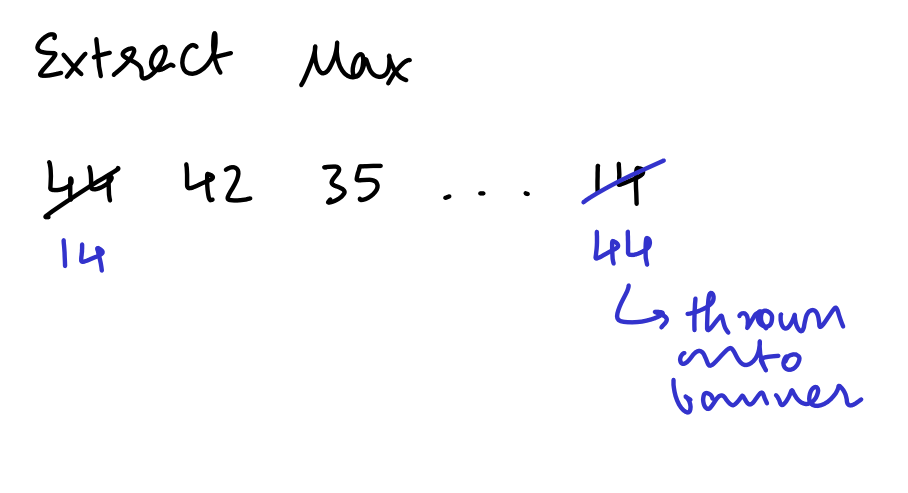
\includegraphics[width=0.8\textwidth]{figures/extractmax.png}
	\caption{figures/extractmax.png}
	\label{fig:Extracting the maximum}
\end{figure}
Consider the figure above. This is what we're doing when we select
the maximum from the array. $44$ and $14$ have been mutually swapped.
But, this destroys the ordering property. 

We can then perform a sequence of operations to fix the order.
\begin{figure}[h]
	\centering
	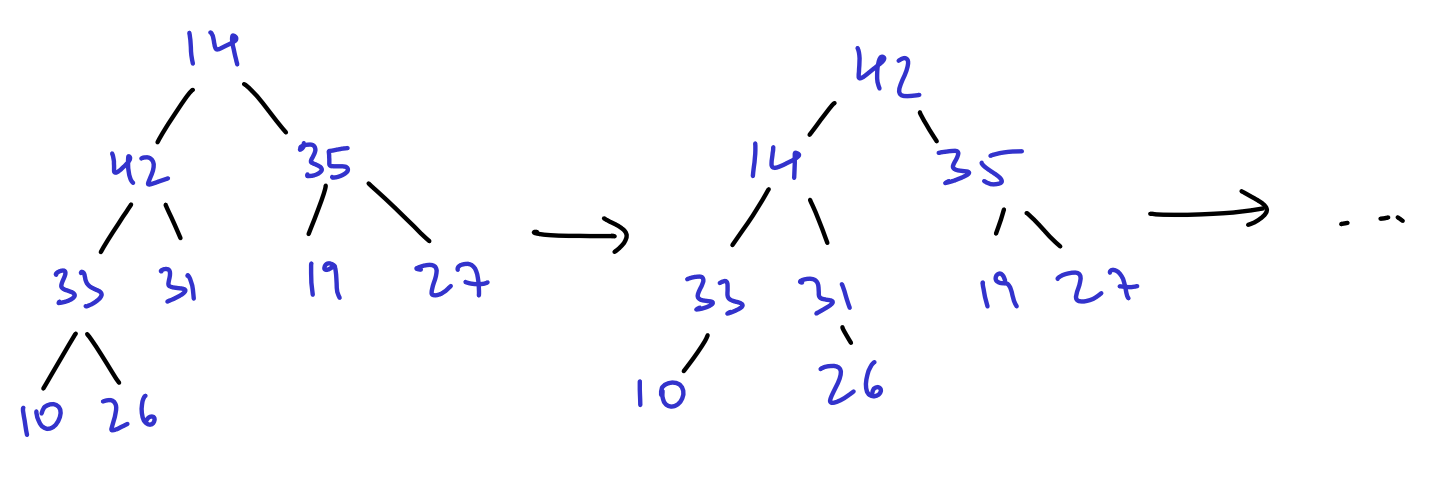
\includegraphics[width=0.8\textwidth]{figures/fix.png}
	\caption{figures/fix.png}
	\label{fig:Fixing the comparison property - propogate down}
\end{figure}
We can keep performing swaps between parent and child as long as we
maintain the invariant that  \texttt{parent} $>$ \texttt{child}.
And because. There will be at most $\log_2n$ comparisons required,
where $n$ is the number of elements in the internal array.

Now, if there is some database trigger and the stack gets updated,
then in general the comparison property will be destroyed. We can
do the same process of sorting them - this time propogating up or
down depending on how the comparisons hold up.

\begin{figure}[h]
	\centering
	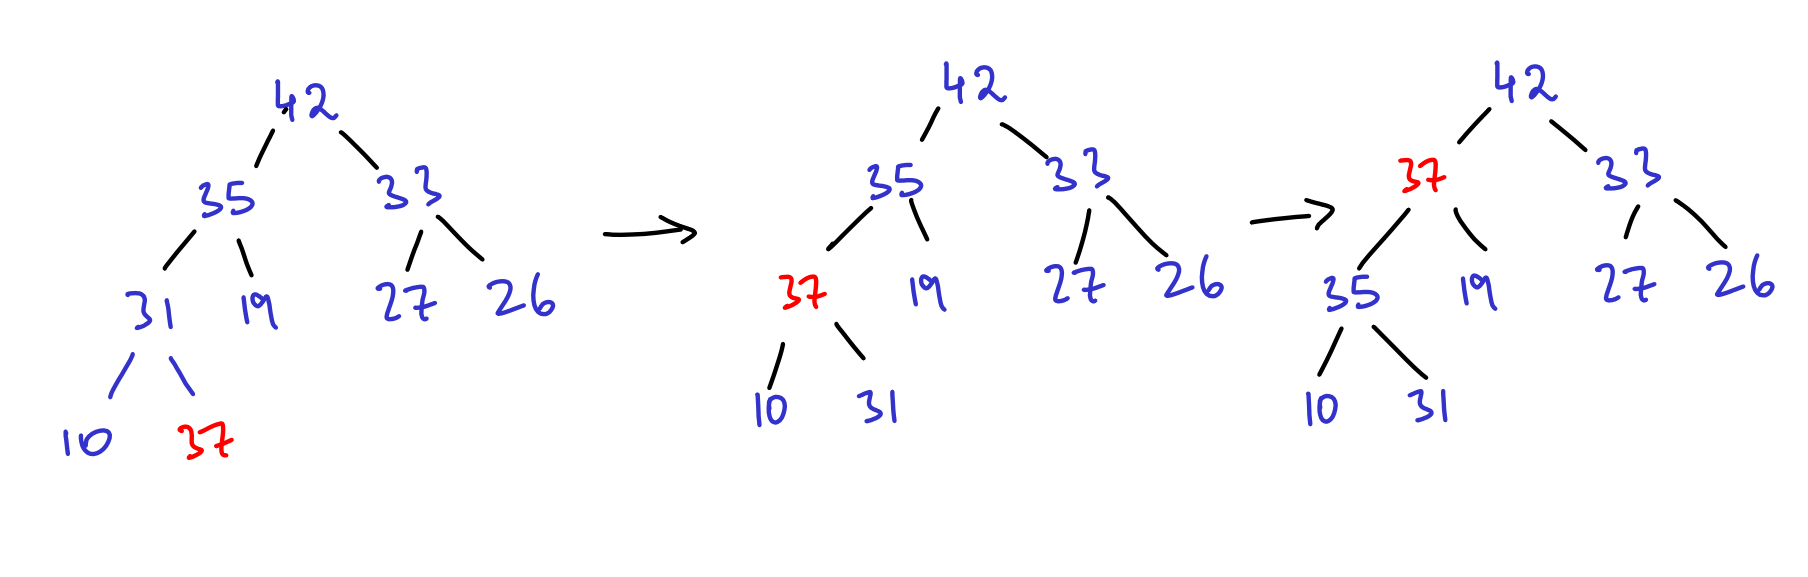
\includegraphics[width=0.8\textwidth]{figures/insertion.png}
	\caption{figures/insertion.png}
	\label{fig: (TODO: verify whether this is right lol) Inserting to heap}
\end{figure}

\textbf{Heap:} a complete binary tree with the comparison property.
Selecting the right data structure is like choosing a scredriver
for a screw that you want to work with. You'd want to choose the best
fit, ya? Don't want to be shoving square cross-sections into triangle
holes.

\section{Recursion}
%%%% TODO: add figures.
\begin{itemize}
	\item Basic idea and basic principle
	\item Parameterization
	\item Computational complexity
	\item Tail recursion
\end{itemize}

\subsection*{Example: Tower of Brahma/Hanoi}
Three rods $A, B, C$, and disks of decreasing size mounted onto the 
rods. Only one disk can be moved from one rod to another in one move 
and a larger disk cannot
be mounted on top of a smaller disk. The objective is to move all the
disks from rod $A$ to rod $B$ while respecting these rules.
A recursive solution for this problem is very simple and elegant.

A recursive solution for a problem of size $n$ requires knowing the
solution to size $n-1$ and then using it to solve the next higher
problem. Also, the program must terminate, so you need a base case.
This whole business is very similar to induction.

The \textbf{base case} here is $n = 1$, in which case we just move
$A \to  B$. This is what the base case would look like in our
coded function.
\begin{code}
\inputminted[samepage=false, breaklines, linenos, firstline=1, lastline=11]{c}{codes/recursion/hanoi.c}
\label{lst:hanoi_basecase}
\caption{Base case of tower of Hanoi problem}
\end{code}

$n=2$ is simple, 
\begin{enumerate}
	\item $A\to C$
	\item  $A\to B$ 
	\item $B\to C$.
\end{enumerate}

Think of the above steps in this way; The first step solves $n=1$ for
rods $A$ and $C$, then we move the next larger disk from $A$ to $B$, and finally the
last step solves the base case for rods  $C$ and $B$, so that the
smaller disk rests on top of the larger one. Take a look at the whole
code
\begin{code}
\inputminted[samepage=false, breaklines, linenos]{c}{codes/recursion/hanoi.c}
\label{lst:hanoi_full}
\caption{Complete solution of tower of Hanoi}
\end{code}

Essentially, this solution first does a bulk move $A\to C$, then moves
the $n ^{\text{th}}$ disk $A\to B$, and then moves the $n-1$ disks 
from $C\to B$.

How does one calculate the total number of moves? We do not have
any explicit loops. Recursive algorithms are best described
using recurrence relations like so
\begin{equation}
	M(n) = 2M(n-1) + 1
\end{equation}
where $M(1) = 1$ is the base case. So, each call does two more calls
and a move. Expanding the recurrence relation, we get
\begin{equation}
	\begin{split}
		M(n) &= 2^{n-1} + \sum_{i=0}^{n-2} 2^{i}\\
		&= 2^{n} - 1
	\end{split}
\end{equation}

Essentially, solving a problem using recursion is about finding
the recurrence relation. Once you have the base case and the
recurrence relation that always reaches the base case, the problem
is pretty much done. The question of correctnes remains, as goes
without saying.

The base case and its termination is very important. Professor
recommends that focus on this first before moving on to the
recurrence relation.

\subsection*{Draw Ruler}
Print the ticks and numbers of a scale (or ruler)
\begin{figure}[h]
	\centering
	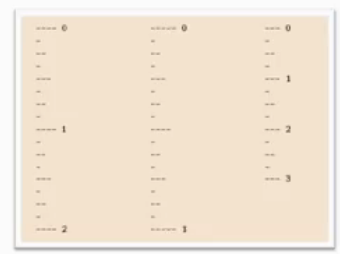
\includegraphics[width=0.5\textwidth]{figures/ruler.png}
	\caption{Sample output of the ruler problem}
	\label{fig:figures-ruler-png}
\end{figure}

So, a ruler is essentially a fractal; zooming in between a pair
of ticks, we see the same pattern again. The ruler is a mix
between two things
\begin{itemize}
	\item Numbered inch markings
	\item Subticks between inch markings, not numbered
\end{itemize}

So, what are we supposed to do?
\begin{itemize}
	\item Identify the recursive structure
	\item identify the base case
	\item complete the base case
	\item solve the problem
\end{itemize}

Our function,  \texttt{drawTicks(length)} takes a single integer,
length of the ticks with inch markings, and prints the ruler of
that tick length.

\emph{Base case:}  \texttt{length == 0}. In this case we draw nothing.
What do the recursive calls look like? We first draw a tick of size
\texttt{length} with label, then draw an interval of center-tick length
\texttt{length - 1} and finally draw another tick of size
\texttt{length} with label.

An interval of a given \texttt{center\_length} has two smaller
intervals before and after it with center-tick length \texttt{center\_length-1}.

I tried to port the lecture's code to CeeLanguage, but there appears
to be some logical error. %%%% TODO: fix
\begin{code}
\inputminted[samepage=false, breaklines, linenos]{c}{codes/recursion/ruler.c}
\label{ruler_c}
\caption{Recursive and helper functions for the ruler problem}
\end{code}
\end{document}
